\documentclass{beamer}

\usepackage{ctex, hyperref}
\usepackage[T1]{fontenc}

%\usepackage[backend=biber,style=authoryear,natbib=true]{biblatex}

% other packages
\usepackage{latexsym,amsmath,xcolor,multicol,booktabs,calligra}
\usepackage{graphicx,pstricks,listings,stackengine}

% \usepackage{cite}


\author{张天山}
\title{Honkai: Star Rail Query System}
\subtitle{数据库课设答辩PPT}
\institute{R成型221-29}
\date{2024年1月15日}
\usepackage{PekingU}

% defs
\def\cmd#1{\texttt{\color{red}\footnotesize $\backslash$#1}}
\def\env#1{\texttt{\color{blue}\footnotesize #1}}
\definecolor{deepblue}{rgb}{0,0,0.5}
\definecolor{deepred}{rgb}{0.6,0,0}
\definecolor{deepgreen}{rgb}{0,0.5,0}
\definecolor{halfgray}{gray}{0.55}

\lstset{
    basicstyle=\ttfamily\small,
    keywordstyle=\bfseries\color{deepblue},
    emphstyle=\ttfamily\color{deepred},    % Custom highlighting style
    stringstyle=\color{deepgreen},
    numbers=left,
    numberstyle=\small\color{halfgray},
    rulesepcolor=\color{red!20!green!20!blue!20},
    frame=shadowbox,
}


\begin{document}

\kaishu
\begin{frame}
    \titlepage
    \begin{figure}[htpb]
        \begin{center}
            %\includegraphics[width=0.2\linewidth]{pic/PKU_logo.png}
        \end{center}
    \end{figure}
\end{frame}

\begin{frame}
    \tableofcontents[sectionstyle=show,subsectionstyle=show/shaded/hide,subsubsectionstyle=show/shaded/hide]
\end{frame}


\section{课题背景与游戏介绍}

\subsection{海报封面}

\begin{frame}{崩坏:星穹铁道}
    \begin{figure}   
        \centering
        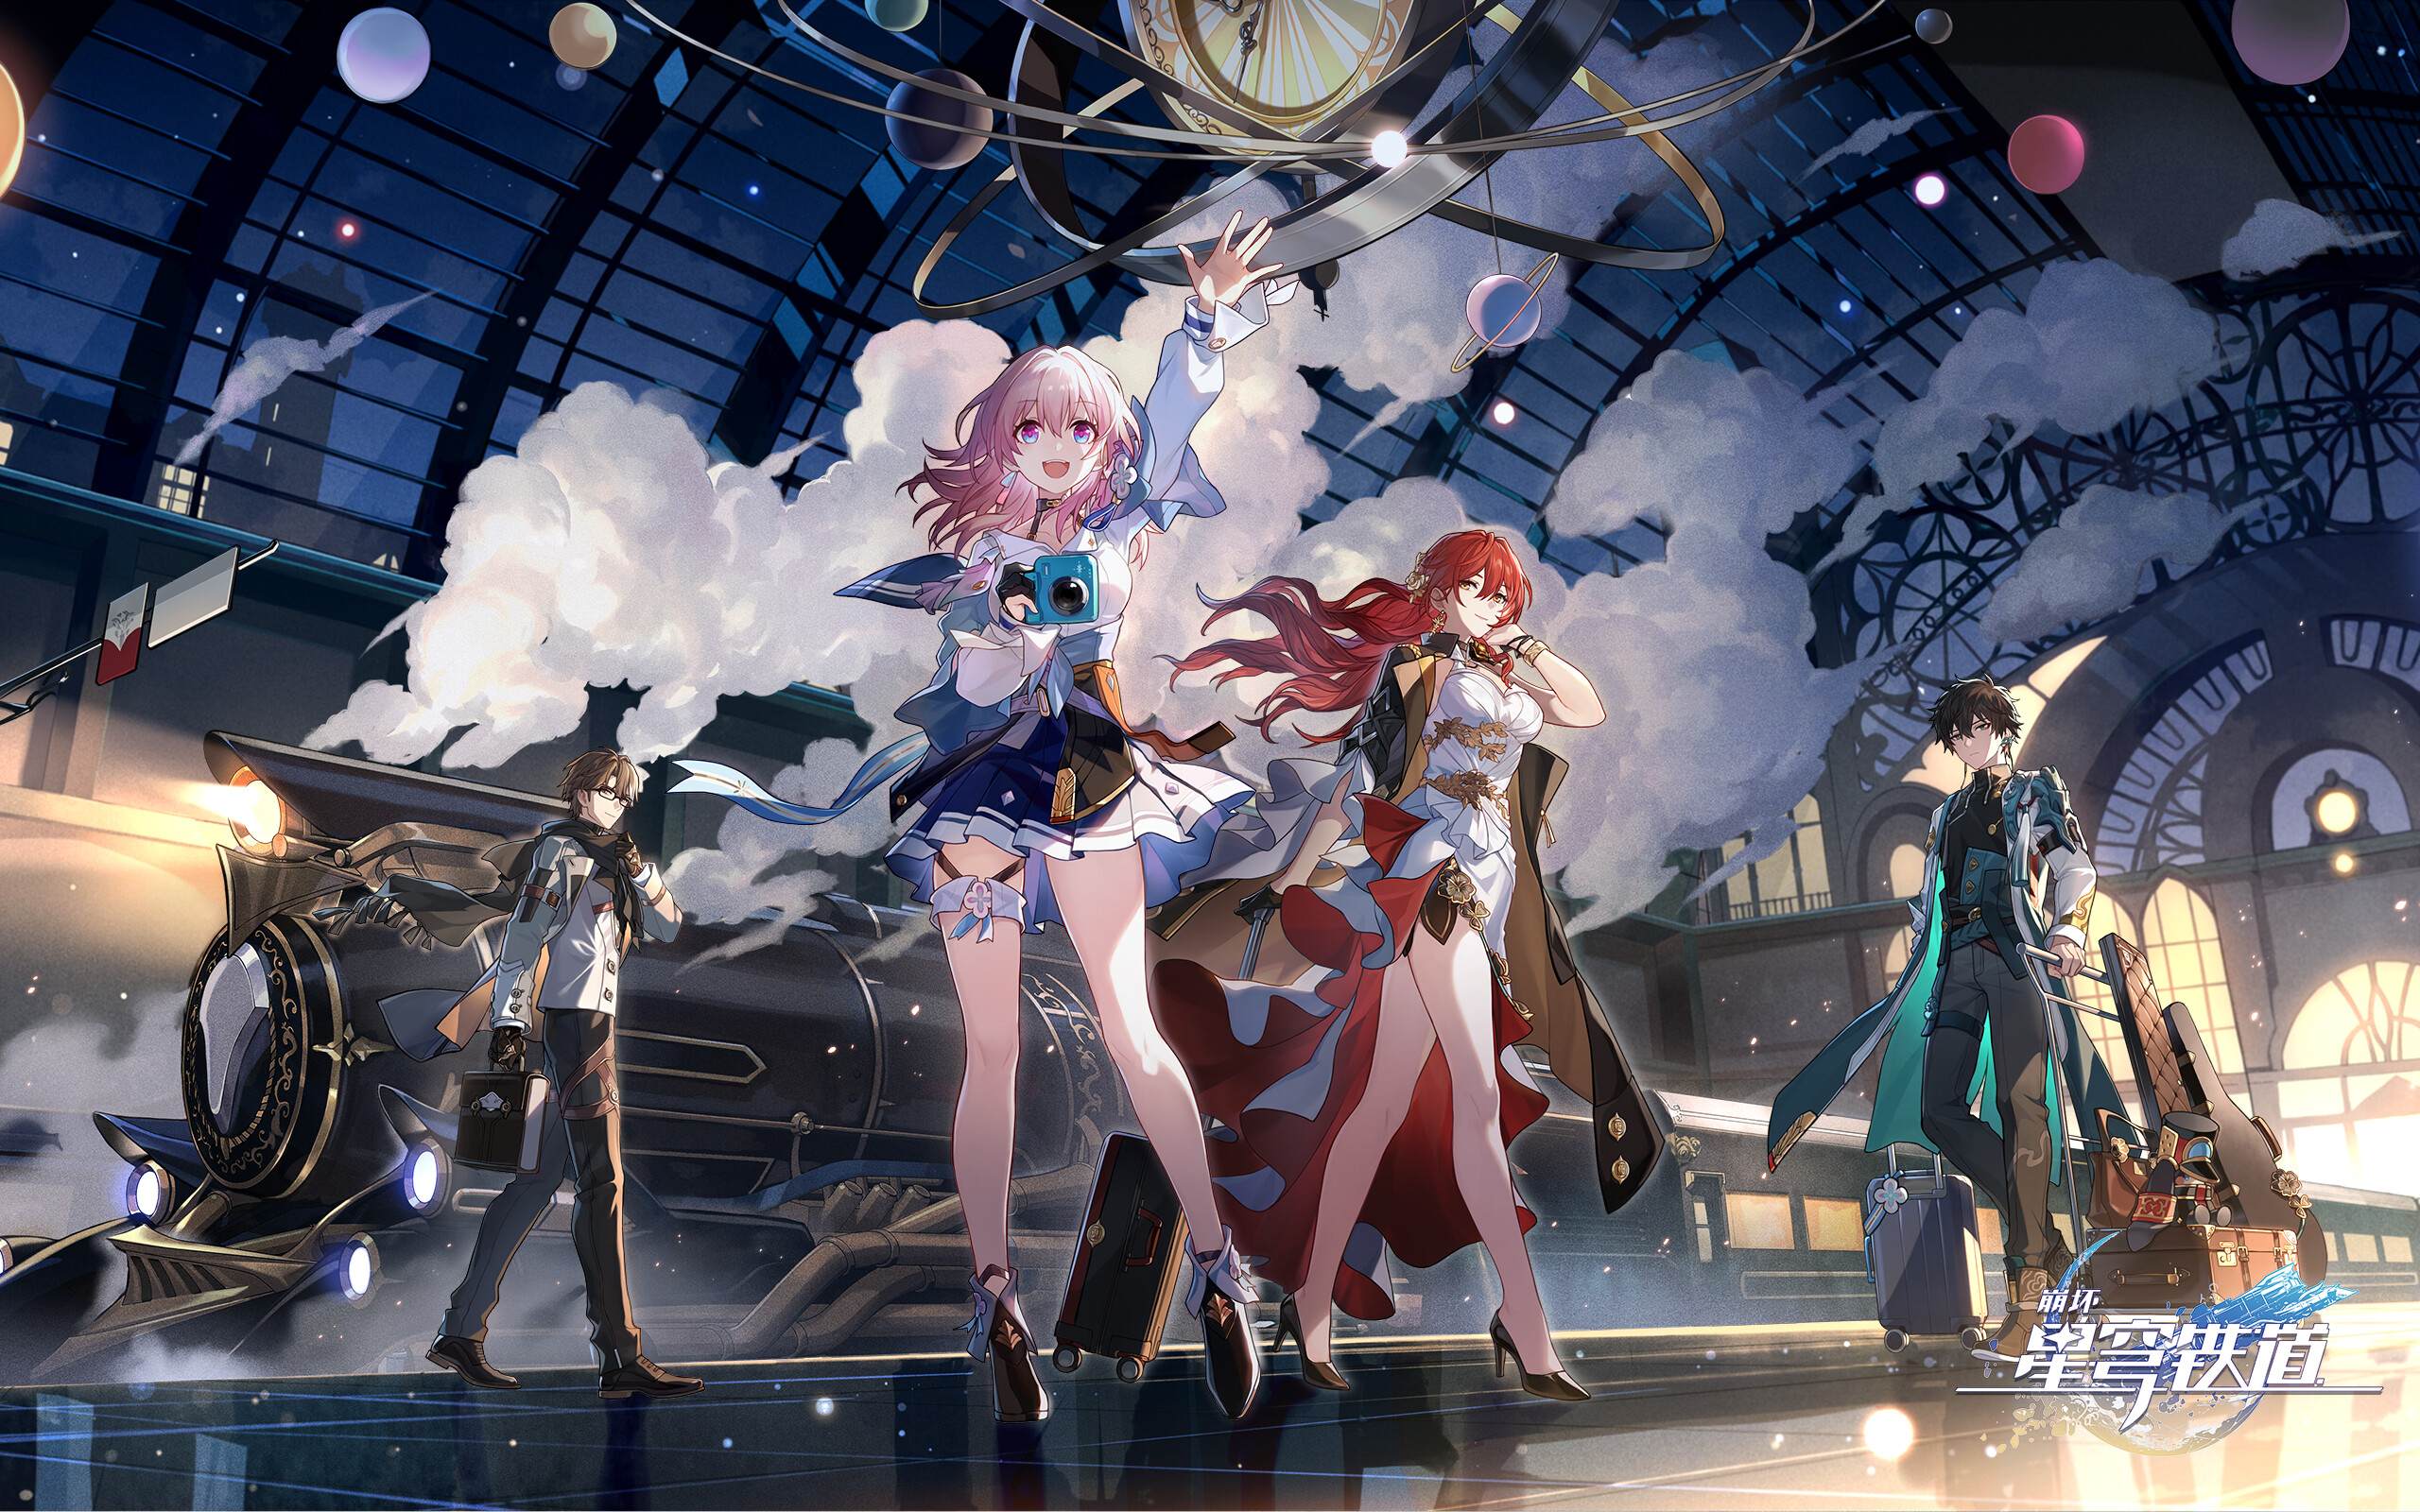
\includegraphics[width=0.9\linewidth]{img/Cover.png} 
        \caption{Honkai:Star Rail 海报\cite{hoyoverse2023honkai}}
        \label{Forward and Reverse Process}
        %\vspace{-0.4cm}
    \end{figure}
\end{frame}



\subsection{游戏介绍}
\begin{frame}{游戏介绍}
    
    崩坏:星穹铁道是米哈游开发的一款回合制角色扮演游戏。作为一款现代化RPG游戏,其具有以下特点:
    \begin{itemize}
        \item 独特的科幻世界观和列车行驶主题
        \item 丰富的养成系统,包括角色、光锥、遗器等多维度培养内容
        \item 深度的战斗策略,需要合理搭配角色阵容和装备
        \item 多样的材料收集与资源管理系统
    \end{itemize}

\end{frame}




\section{问题提出}

\subsection{刷材料?刷副本?每天应该怎么分配体力?}

\begin{frame}
    
    我们在游玩星穹铁道这款游戏的时候,往往需要刷光锥,刷升级材料,刷遗器,玩家需要合理规划资源来培养角色,提高战斗力,因为数据量太大,所以出现了以下这些问题:
    \begin{itemize}
        \item 游戏内容繁多,玩家难以快速找到所需信息
        \item 培养材料分散在多个获取渠道
        \item 角色培养路线规划困难
        \item 缺乏系统化的数据查询工具
    \end{itemize}
\end{frame}

\subsection{设想解决办法}
\begin{frame}
    面对以上问题,我结合这次数据库课设,做出了一个简易的查阅资料数据库:
    \begin{itemize}
        \item 支持材料规划功能
        \item 实现数据之间的关联查询
        \item 建立统一的数据管理系统
        \item 在后续使用后端框架完善系统
    \end{itemize}
\end{frame}



\section{解决办法:数据库设计}

\subsection{游戏内容解释}

\begin{frame}{人物 Characters}
    \begin{figure}   
        \centering
        \includegraphics[width=0.8\linewidth]{img/ebba9a3133c78f8cd6f6b04e754b4b4.jpg} 
        \caption{人物展示,人物有等级上限,需要对应材料升级}
        \label{Forward and Reverse Process}
        %\vspace{-0.4cm}
        \end{figure}
\end{frame}

\begin{frame}{命途 Paths}
    \begin{figure}   
        \centering
        \includegraphics[width=0.8\linewidth]{img/ecf27237569fe3ffe1d582150f50fe1.jpg} 
        \caption{命途解释}
        \label{Forward and Reverse Process}
        %\vspace{-0.4cm}
        \end{figure}
\end{frame}

\begin{frame}{技能 Skills}
    \begin{figure}   
        \centering
        \includegraphics[width=0.8\linewidth]{img/1f42c223f24df3012cd99b9a04b29ec.jpg} 
        \caption{技能升级材料介绍}
        \label{Forward and Reverse Process}
        %\vspace{-0.4cm}
        \end{figure}
\end{frame}

\begin{frame}{光锥 LightCones }
    \begin{figure}   
        \centering
        \includegraphics[width=0.8\linewidth]{img/446bed7251f535d2899f540d27a7fa2.jpg} 
        \caption{光锥展示,光锥有等级上限,需要对应材料升级}
        \label{Forward and Reverse Process}
        %\vspace{-0.4cm}
        \end{figure}
\end{frame}



\begin{frame}{遗器套装 RelicSets}
    \begin{figure}
        \centering
        \begin{minipage}[c]{0.48\textwidth}
            \centering
            \includegraphics[width=\textwidth, height=0.7\textheight, keepaspectratio]{img/17a0984074ed94a8bef60ce68ae7e3e.jpg}
        \end{minipage}
        \hfill  % 水平间距
        \begin{minipage}[c]{0.48\textwidth}
            \centering
            \includegraphics[width=\textwidth, height=0.7\textheight, keepaspectratio]{img/13c8cb9f4c585da93f382f1c3273bb5.jpg}
        \end{minipage}
        \caption{不同的人物可以根据不同的套装提高自己的上限}
        \label{fig:characters}
    \end{figure}
\end{frame}



\begin{frame}{遗器 Relics}
    \begin{figure}   
        \centering
        \includegraphics[width=0.8\linewidth]{img/e6e4bfd527b9df53ecc28ae6dd85f8c.jpg} 
        \caption{遗器升级需要对应的升级材料}
        \label{Forward and Reverse Process}
        %\vspace{-0.4cm}
        \end{figure}
\end{frame}

\begin{frame}{材料 Materials }
    \begin{figure}   
        \centering
        \includegraphics[width=0.8\linewidth]{img/a215e476d58dc40630e6ce622285496.jpg} 
        \caption{用于升级人物,光锥,遗器的各种材料}
        \label{Forward and Reverse Process}
        %\vspace{-0.4cm}
        \end{figure}
\end{frame}

\begin{frame}{敌人 Enemies}
    \begin{figure}   
        \centering
        \includegraphics[width=0.8\linewidth]{img/8e695de707f7e1c40f78bd780b33f7a.jpg} 
        \caption{不同的敌人会掉落不同的升级材料用于给不同命途的角色升级}
        \label{Forward and Reverse Process}
        %\vspace{-0.4cm}
        \end{figure}
\end{frame}


\subsection{实体介绍}
\begin{frame}{数据库表设计}
    % 使用 beamercolorbox 创建更美观的表格
    \begin{columns}[T]
        % 第一列
        \begin{column}{0.25\textwidth}
            \begin{beamercolorbox}[rounded=true,shadow=true]{block title}
                \centering\textbf{Paths \\命途}
            \end{beamercolorbox}
            \begin{beamercolorbox}[rounded=true]{block body}
                \footnotesize
                \textcolor{blue}{path\_id} \\
                path\_name \\
                description \\
            \end{beamercolorbox}
            
            \vspace{0.85cm}
            
            \begin{beamercolorbox}[rounded=true,shadow=true]{block title}
                \centering\textbf{RelicSets \\遗器套装}
            \end{beamercolorbox}
            \begin{beamercolorbox}[rounded=true]{block body}
                \footnotesize
                \textcolor{blue}{set\_id} \\
                set\_name \\
                effects
            \end{beamercolorbox}
        \end{column}
        
        % 第二列
        \begin{column}{0.25\textwidth}
            \begin{beamercolorbox}[rounded=true,shadow=true]{block title}
                \centering\textbf{Characters \\角色}
            \end{beamercolorbox}
            \begin{beamercolorbox}[rounded=true]{block body}
                \footnotesize
                \textcolor{blue}{char\_id} \\
                char\_name \\
                \textcolor{red}{path\_id} \\
                rarity
            \end{beamercolorbox}
            
            \vspace{0.5cm}
            
            \begin{beamercolorbox}[rounded=true,shadow=true]{block title}
                \centering\textbf{Relics \\遗器}
            \end{beamercolorbox}
            \begin{beamercolorbox}[rounded=true]{block body}
                \footnotesize
                \textcolor{blue}{relic\_id} \\
                \textcolor{red}{set\_id} \\
                main\_stat
            \end{beamercolorbox}
        \end{column}
        
        % 第三列
        \begin{column}{0.25\textwidth}
            \begin{beamercolorbox}[rounded=true,shadow=true]{block title}
                \centering\textbf{Skills \\技能}
            \end{beamercolorbox}
            \begin{beamercolorbox}[rounded=true]{block body}
                \footnotesize
                \textcolor{blue}{skill\_id} \\
                \textcolor{red}{char\_id} \\
                skill\_name \\
                skill\_type
            \end{beamercolorbox}
            
            \vspace{0.5cm}
            
            \begin{beamercolorbox}[rounded=true,shadow=true]{block title}
                \centering\textbf{Materials \\材料}
            \end{beamercolorbox}
            \begin{beamercolorbox}[rounded=true]{block body}
                \footnotesize
                \textcolor{blue}{material\_id} \\
                material\_name \\
                material\_type
            \end{beamercolorbox}
        \end{column}
        
        % 第四列
        \begin{column}{0.25\textwidth}
            \begin{beamercolorbox}[rounded=true,shadow=true]{block title}
                \centering\textbf{LightCones \\光锥}
            \end{beamercolorbox}
            \begin{beamercolorbox}[rounded=true]{block body}
                \footnotesize
                \textcolor{blue}{cone\_id} \\
                cone\_name \\
                \textcolor{red}{path\_id} \\
                rarity
            \end{beamercolorbox}
            
            \vspace{0.5cm}
            
            \begin{beamercolorbox}[rounded=true,shadow=true]{block title}
                \centering\textbf{Enemies \\敌人}
            \end{beamercolorbox}
            \begin{beamercolorbox}[rounded=true]{block body}
                \footnotesize
                \textcolor{blue}{enemy\_id} \\
                enemy\_name \\
                enemy\_type
            \end{beamercolorbox}
        \end{column}
    \end{columns}
    
    \vspace{0.3cm}
    \begin{beamercolorbox}[rounded=true,shadow=true]{block body}
        \centering\footnotesize
        \textcolor{blue}{蓝色} = 主键 \hspace{1cm} 
        \textcolor{red}{红色} = 外键
    \end{beamercolorbox}
\end{frame}


\subsection{E-R图设计}

\begin{frame}[fragile]{Mermaid}
    \begin{minipage}{0.55\linewidth}
\begin{lstlisting}[]
erDiagram
    // 连接信息
    Paths ||--o{ Charact
    ers : "has"
    Paths ||--o{ LightCo
    nes : "restricts"
    Characters ||--o{ Sk
    ills : "has"
    ....
    // 自身信息
    Paths {
        int path_id PK
        string path_name
        datetime updated_at
        .....
    }
\end{lstlisting}
    \end{minipage}\hspace{1cm}
    \begin{minipage}{0.3\linewidth}
        \begin{itemize}
            \item 快速进行图表更新
            \item 智能调整实体位置
            \item 设计信息太多可以快速整理(都是代码不用重新查找)
            
        \end{itemize}
    \end{minipage}
    \medskip
\end{frame}


\begin{frame}{E-R图展示}
    \begin{itemize}[<+-| alert@+>] 
        \begin{figure}   
        \centering
        \includegraphics[width=1\linewidth]{img/image.png} 
        \caption{E-R图展示}
        \label{Forward and Reverse Process}
        \vspace{-0.4cm}
        \end{figure}
    \end{itemize}
\end{frame}


\begin{frame}{关系介绍}
\centering
命途 1:N 角色/光锥\\
\vspace{0.4cm}
角色 1:N 技能\\
\vspace{0.4cm}
角色/光锥 N:N 材料\\
\vspace{0.4cm}
遗器 N:1 遗器套装\\
\vspace{0.4cm}
敌人 1:N 材料

\end{frame}




\subsection{设计亮点}

\begin{frame}[fragile]{游戏核心数据表设计}
    \begin{minipage}{0.6\linewidth}
\begin{lstlisting}[language=sql]
CREATE TABLE Characters (
    character_id INT PRIMARY
    KEY IDENTITY(1,1),
    character_name NVARCHAR
    (100)
    NOT NULL UNIQUE,
    rarity INT CHECK (rarity 
    BETWEEN 4 AND 5),
    ...
)

\end{lstlisting}
    \end{minipage}\hspace{0.5cm}
    \begin{minipage}{0.25\linewidth}
        \begin{itemize}
            \item 使用CHECK约束实现游戏规则
            \item UNIQUE约束防止重复数据
            
        \end{itemize}
    \end{minipage}
    \medskip
\end{frame}



\begin{frame}[fragile]{关联系统设计}
    \begin{minipage}{0.6\linewidth}
\begin{lstlisting}[language=sql]

CREATE TABLE Skills (
    skill_id INT PRIMARY KEY 
    IDENTITY(1,1),
    character_id INT FOREIGN 
    KEY REFERENCES Characters
    (character_id),
    skill_type NVARCHAR(20) 
    CHECK (skill_type IN 
    ('普攻', '战技', '终结技',
    '天赋', '秘技')),
    ...
)

\end{lstlisting}
    \end{minipage}\hspace{0.5cm}
    \begin{minipage}{0.25\linewidth}
        \begin{itemize}
            \item 技能类型限制
            \item 模块化设计
            
        \end{itemize}
    \end{minipage}
    \medskip
\end{frame}



\begin{frame}[fragile]{智能查询系统}
    \begin{minipage}{0.6\linewidth}
\begin{lstlisting}[language=sql]
CREATE PROCEDURE GetChara
cterFullInfo
    @character_id INT = NULL,
    @character_name 
    NVARCHAR(100) = NULL
\end{lstlisting}
    \end{minipage}\hspace{0.5cm}
    \begin{minipage}{0.25\linewidth}
        \begin{itemize}
            \item 支持多参数查询
            \item 完整的错误处理和灵活的查询条件
            
        \end{itemize}
    \end{minipage}
    \medskip
\end{frame}


\begin{frame}[fragile]{数据统计分析}
    \begin{minipage}{0.6\linewidth}
\begin{lstlisting}[language=sql]
CREATE VIEW Character
Statistics AS
SELECT 
    p.path_name,
    COUNT(*) as character
    _count,
    AVG(CAST(c.rarity as 
    FLOAT)) as avg_rarity
\end{lstlisting}
    \end{minipage}\hspace{0.5cm}
    \begin{minipage}{0.25\linewidth}
        \begin{itemize}
            \item 多表关联查询
            \item 命途分布分析
            
        \end{itemize}
    \end{minipage}
    \medskip
\end{frame}




\section{使用方式}
\begin{frame}{文件介绍}
    \begin{itemize}
        \item {create database}创建基本表结构
        \item {create procedures}数据库的功能性组件创建文件,包括触发器,存储过程,视图,索引
    \end{itemize}
\end{frame}

\section{参考文献}

\begin{frame}
 \frametitle{References}
 \bibliography{ref}
 %\bibliographystyle{alpha}
\end{frame}

\begin{frame}
    \begin{center}
    {\Huge 愿此行,终抵群星!}\\
    \vspace{0.9cm}
        {\Huge\calligra Thanks!}
    \end{center}
\end{frame}

\end{document}
